\documentclass[twocolumn]{aastex631}

% Suppress the "Draft version / Typeset using" banner.
\makeatletter
\long\def\frontmatter@title@above{}
\makeatother

\usepackage{graphicx}
\usepackage{amsmath}
\usepackage{url}
\usepackage{xcolor}
\usepackage{tikz}
\usetikzlibrary{calc,fit,positioning,arrows.meta,backgrounds,shapes.geometric}
\definecolor{oiGreen}{HTML}{009E73}
\definecolor{oiOrange}{HTML}{D55E00}
\definecolor{oiBlue}{HTML}{0072B2}
\definecolor{oiGray}{HTML}{4D4D4D}


\usepackage{lettrine}

\newlength{\pixunit}
\setlength{\pixunit}{4.2pt}
\newsavebox{\pixelAbox}
\savebox{\pixelAbox}{%
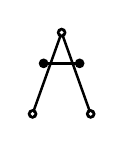
\begin{tikzpicture}[x=\pixunit,y=\pixunit,line width=0.9pt]
  \draw[] (0,-7) -- (2.5,0) -- (5,-7);
  \draw[] (0.95,-2.65) -- (4.05,-2.65);
  \foreach \p in {(0,-7),(2.5,0),(5,-7),(0.95,-2.65),(4.05,-2.65)}
    \fill[] \p circle (0.42);
  \foreach \p in {(0,-7),(2.5,0),(5,-7)}
    \fill[white] \p circle (0.17);
\end{tikzpicture}}
\newcommand{\pixelA}{\usebox{\pixelAbox}}

% auto-generated by src/s8_fill_numbers.py; do not edit
\newcommand{\anchorRangeControls}{1.05--1.2}
\newcommand{\anchorRangeMarkers}{2.6--6.8}
\newcommand{\betaMarkersAbs}{13.6\%}
\newcommand{\betaMarkersFull}{47\%}
\newcommand{\bottomTopicName}{instrumentation}
\newcommand{\boundaryShift}{4 percentage points}
\newcommand{\ctrlBetaAbs}{22\%}
\newcommand{\ctrlBetaFull}{51\%}
\newcommand{\ctrlExcessRate}{26\%}
\newcommand{\ctrlModelPi}{$56^{+4}_{-4}$\%}
\newcommand{\declCountsByYear}{26, 38, 153, and 175}
\newcommand{\declRateTwentyFive}{0.81\%}
\newcommand{\declRateTwentySix}{2.07\%}
\newcommand{\deltaEarly}{3.5}
\newcommand{\deltaLate}{1.5}
\newcommand{\disclosureGapFactor}{$\sim$66}
\newcommand{\disclosureGapFactorTwentySix}{$\sim$42}
\newcommand{\gammaShift}{22 percentage points}
\newcommand{\gammaShiftDown}{4 percentage points}
\newcommand{\gammaShiftUp}{22 percentage points}
\newcommand{\ladderAbsRungFour}{$61^{+13}_{-12}$\%}
\newcommand{\ladderAbsRungThree}{79\%}
\newcommand{\ladderAbsRungTwo}{83\%}
\newcommand{\ladderAbsRungZero}{13.6\%}
\newcommand{\ladderCtrlRungFour}{unid.}
\newcommand{\ladderCtrlRungZero}{51\%}
\newcommand{\ladderFullRungFour}{$54^{+8}_{-8}$\%}
\newcommand{\ladderFullRungThree}{56\%}
\newcommand{\ladderFullRungTwo}{61\%}
\newcommand{\ladderFullRungZero}{47\%}
\newcommand{\markerExcessRate}{81\%}
\newcommand{\markerRiseAbs}{3.3}
\newcommand{\markerRiseFulltext}{2.6}
\newcommand{\monotoneShift}{0 percentage points}
\newcommand{\nAbstracts}{233{,}428}
\newcommand{\nDeclared}{400}
\newcommand{\nDeclaredCohort}{392}
\newcommand{\nDeclaredPreChatGPT}{0}
\newcommand{\nDeclaredTwentyFive}{155}
\newcommand{\nExpandedHeld}{32}
\newcommand{\nExpandedNew}{30}
\newcommand{\nExpandedWords}{34}
\newcommand{\nFulltext}{207{,}111}
\newcommand{\nFulltextRaw}{219,434}
\newcommand{\noDisclosureShift}{10 percentage points}
\newcommand{\observedExcess}{2.4}
\newcommand{\piAbstractsCohort}{$75^{+16}_{-16}$\%}
\newcommand{\piAbstractsHeadline}{$61^{+13}_{-12}$\%}
\newcommand{\piAbstractsNuts}{$61^{+13}_{-12}$\%}
\newcommand{\piBottomClass}{44\%}
\newcommand{\piExpandedHeadline}{$79^{+11}_{-11}$\%}
\newcommand{\piExpandedTracked}{87\%}
\newcommand{\piFulltextBracket}{54--80\%}
\newcommand{\piFulltextHeadline}{$54^{+8}_{-8}$\%}
\newcommand{\piFulltextLaplace}{$67^{+13}_{-11}$\%}
\newcommand{\piFulltextTwentyFour}{$20^{+3}_{-3}$\%}
\newcommand{\piFulltextTwentySix}{$87^{+8}_{-10}$\%}
\newcommand{\piGridFloor}{36\%}
\newcommand{\piGridFloorTwentySix}{64\%}
\newcommand{\piGridRange}{50--87\%}
\newcommand{\piHeadlinePM}{$54^{+8}_{-8}\,(\mathrm{stat},\,95\%)\,^{+26}_{-0}\,(\mathrm{sys,\ background})$}
\newcommand{\piHeadlinePMTwentySix}{$87^{+8}_{-10}\,(\mathrm{stat},\,95\%)\,^{+12}_{-0}\,(\mathrm{sys,\ background})$}
\newcommand{\piStatOneSigma}{$^{+4}_{-4}$}
\newcommand{\piStatOneSigmaTwentySix}{$^{+5}_{-5}$}
\newcommand{\piTopClass}{65\%}
\newcommand{\piUnconstrained}{53\%}
\newcommand{\piWeightShift}{1.7 percentage points}
\newcommand{\piWholeBody}{$52^{+7}_{-7}$\%}
\newcommand{\topTopicName}{cosmology}


\shorttitle{Most recent astronomy papers use language-model assistance}
\shortauthors{Saad \& Ting}

\begin{document}

\title{More than half of recent astronomy papers are being written with
language-model assistance}

\author[0009-0004-9592-2311]{Serat M. Saad}
\affiliation{Department of Astronomy, The Ohio State University, 140 West 18th
Avenue, Columbus, OH 43210, USA}

\author[0000-0001-5082-9536]{Yuan-Sen Ting}
\affiliation{Department of Astronomy, The Ohio State University, 140 West 18th
Avenue, Columbus, OH 43210, USA}
\affiliation{Center for Cosmology and AstroParticle Physics (CCAPP), The Ohio
State University, Columbus, OH 43210, USA}
\affiliation{Max-Planck-Institut f\"ur Astronomie, K\"onigstuhl 17, D-69117
Heidelberg, Germany}

\begin{abstract}
Since the public announcement of ChatGPT in 2022, large language models have been used in the writing of literature in every scientific field. In this work, we measure how much of the astronomy literature is now written with the help of language models. From the full text of \nFulltext\ astro-ph papers, spanning 2015 to mid-2026, we count the vocabulary that language models favor to calibrate its usage on the \nDeclared\ papers whose authors disclosed model use. We then infer the fraction of assisted papers with a hierarchical Bayesian model. The model uses the disclosed papers to fix the marker rate of assisted prose and the 106{,}000 papers in the corpus that predate ChatGPT to fix the rate without assistance. No data can tell us how the unassisted rate would have continued after 2022, had chatbots never been released, so rather than assuming a single continuation we fit three, and together they give the plausible range. For 2025, the primary specification gives \piFulltextHeadline, and the three continuations span \piFulltextBracket. The fraction stays at or above \piGridFloor\ under every variant we tried. We conclude that more than half of recent astro-ph papers carry a language-model trace in their prose, while only \declRateTwentyFive\ declare it.
\end{abstract}

\keywords{Astronomy data analysis (1858) --- Publishing (1329) ---
Bayesian statistics (1900)}
% =====================================================================
\section{Introduction}\label{sec:intro}
\lettrine[lines=2, findent=3pt, nindent=0pt, slope=0pt, ante=]{\pixelA}{}%
fter ChatGPT (Chat Generative Pre-trained Transformer) became publicly available in November 2022, a specific set of English words has spread through scientific writing. These words are not technical terms rather they are stylistic choices, like \textit{delve}, \textit{underscore}, \textit{intricate}, \textit{pivotal}, and their relatives, that language models favor and that human writers before November 2022 used rarely. The models are transformer language models \citep{Vaswani2017} scaled to the point where fluent scientific prose costs nothing to generate \citep{Brown2020}. The pattern was first quantified by \citet{Gray2025}, who estimated from keyword frequencies that at least one percent of 2023 articles were model-assisted, and by \citet{Liang2024}, who fitted a distributional model to abstracts and found rates of a few percent, rising fastest in computer science. \citet{Kobak2024} then introduced the approach that now dominates the field. Rather than assume a word list, they measured which words rose anomalously across 14 million PubMed abstracts and concluded that at least 10\% of 2024 biomedical abstracts had been processed with a language model. Extending the method to 1.2 million biomedical full texts, \citet{Holzwarth2026} report that 89\% of papers showed excess model-associated vocabulary by late 2025. Related measurements now exist for peer-review text \citep{Liang2024review}, for condensed-matter physics \citep{Xu2024}, and for preprints across arXiv \citep{Juzek2025, Bao2025}.

Although the counting of excess vocabulary is more straightforward, converting a count into a statement of the form ``$x$ per cent of papers used a language model'' is not, and the obstacle is not statistical noise. With hundreds of thousands of papers the observed word frequencies are known almost exactly. The obstacle is that the inference requires the frequency these words would have had if language models had never been released. This is something that stopped being observable in November 2022. Every estimate in this literature depends on a counterfactual that no amount of data can measure.

Existing estimators handle that counterfactual by fixing it. The excess-vocabulary bound of \citet{Kobak2024} subtracts a baseline frequency from the observed one and reports the difference as a floor. The extrapolation estimator of \citet{Holzwarth2026} fits the pre-2022 trend of each marker word, extends it linearly, and converts the excess into an estimate that is unbiased if the extension is correct. None of these approach reports uncertainty on the extension itself, and both share three further restrictions that are rarely stated. Each paper is reduced to a binary flag, so a 200-word abstract and a 15{,}000-word monograph count equally. The background is one number per year, so no allowance is made for documents growing longer or for topics drifting. And the excess rate of assisted prose is held fixed, so the method cannot separate more papers using models from models becoming harder to detect, a failure mode the literature has already recorded, since \citet{Geng2025} showed that \textit{delve} fell sharply once it became famous in early 2024 while other model-favored words kept rising, so authors adapt and any fixed vocabulary loses power with time. The same group documented the initial shift a year earlier \citep{Geng2024}. The question matters because the documented failure modes of unsupervised model use are concrete, most obviously fabricated references \citep{Walters2023, Topaz2026}, and because researchers themselves are split on whether such use is acceptable \citep{Kwon2025}. Many journals also ask for disclosure, so it is worth knowing how much goes undisclosed.

No comparable measurement exists for astronomy, mainly because no clean full-text corpus existed. That changed with the AstroMLab~5 catalog \citep{Ting2025}, which provides uniform, OCR-normalized full text for 433{,}176 astro-ph papers through August 2026, together with abstracts and topic assignments. We work from the full text rather than the abstracts. An abstract offers a few hundred tokens of evidence, most containing no marker at all, while a paper body offers thousands.

In this paper we make the measurement with a hierarchical bayesian model. We calibrate the background rate of marker words on the pre-ChatGPT era and the assisted rate on the papers whose authors state that they used a model, and we report the population fraction as the mixture weight. Where the data cannot decide between assumptions we fit the alternatives rather than choose one, and we quote the conservative end of the resulting range. Under the primary specification we obtain a 2025 assisted fraction of \piFulltextHeadline, and across every variant we ran, spanning the background counterfactual, the monotonicity assumption, the marker vocabulary, and the calibration, our estimate never falls below \piGridFloor.

In Section~\ref{sec:methods} we describe the corpus, the vocabulary, the declarations, and the model. In Section~\ref{sec:results} we report the assisted fraction and the checks that constrain it, including a control test that the standard estimator fails on this corpus. In Section~\ref{sec:discussion} we compare the result with biomedicine and set
out what we think follows.

% =====================================================================
\section{Methods}\label{sec:methods}

\subsection{Corpus and cohort}\label{sec:m-corpus}

We take all text from the AstroMLab~5 catalog \citep{Ting2025}. We date every paper by its first submission and decoded from the arXiv identifier so that a paper posted in 2019 and revised in 2024 cannot carry post-ChatGPT text into the pre-ChatGPT era. The OCR text corresponds to the latest revision, so a small amount of such leakage remains possible. We bound it in Section~\ref{sec:m-robust} by moving the boundary.

We lowercase the text and tokenize it on contiguous alphabetic strings. We remove tables, displayed and inline mathematics, URLs, figure placeholders, and affiliation lines. We then segment the body on section headers into introduction, methods and data, results, discussion, and conclusions, and we analyze only these five section groups. We exclude the abstract so that our full-text analysis does not re-read the same prose, and we exclude
references, acknowledgments, and appendices because their vocabulary is formulaic. We also exclude the unlabeled remainder of the body, which shrinks from half of the body in 2015 to two-fifths in 2026 as OCR sectioning improves. Including it would fold that change in composition into the language signal. We require at least 300 analyzed tokens and a topic assignment, which leaves \nFulltext\ papers first submitted between January 2015 and June 2026, with a median of about 2{,}500 analyzed tokens.

\subsection{Marker, control, and null vocabulary}\label{sec:m-words}

We count three baskets per paper and per section. The marker basket is 38 words that we take from the published biomedical and computer-science lists \citep{Liang2024, Kobak2024, Gray2025}, split between rare, high-specificity words such as \textit{delve} and \textit{underscore} and commoner ones such as \textit{comprehensive} and \textit{notably}. The control basket is ten neutral astronomy content words, among them \textit{observed}, \textit{galaxy}, and \textit{redshift}, that no language model has any reason to favor. The null basket is fifteen common hedges and intensifiers with pre-2020 frequencies comparable to those of the marker words. Table~\ref{tab:baskets} lists both marker baskets in full, together with the control and null vocabularies.

We pass the controls and the nulls through the identical pipeline at every stage. Any prevalence they generate measures our own systematic error rather than language-model use, and we report it in those terms. We treat this as our main diagnostic, and in Section~\ref{sec:placebo} we show that the document-frequency estimator does not survive it at full-text lengths.

\subsection{Declarations of model use}\label{sec:m-decl}

A small number of authors state in the paper that they used a language model. We scan every full text for a single sentence that joins a named tool or an explicit language-model phrase, writing or editing vocabulary, and an authorial-use construction such as ``we used'' or ``the authors acknowledge''. We exclude papers about language models with a mention-count veto. We also handle two astronomy-specific ambiguities, the Gemini telescopes and colleagues named Claude, by requiring a vendor or version qualifier before we accept an ambiguous name.

We find \nDeclared\ declarations. None fall before 2023, and the counts for 2023 through mid-2026 are 29, 52, 200, and 104. The pre-2023 null constrains our false-alarm rate, because the corpus offers roughly 160{,}000 earlier opportunities to false-alarm and the detector triggers on none of them. Declared papers use marker vocabulary at \anchorRangeMarkers\ times the background rate and control vocabulary at the background rate. We use that contrast to
calibrate the model.

We audited the detector for missed declarations with a language-model judge.
We drew 150 undeclared papers from 2024--2026 at random, screened the closing
3{,}500 characters of each for any loose model-related term, and read the
three candidates that surfaced in full. None is a declaration, since two are
funding-program and compute-cluster names that contain the letters AI and one
is a paper about language models that the mention-count veto already handles.
Zero misses in 150 papers bounds the false-negative rate below 2\% of papers
at 95\% confidence. We re-read 20 declared papers the same way, and every
statement visible in the closing text is a genuine authorial declaration,
almost all naming grammar, clarity, or language editing as the purpose.

\subsection{The mixture model}\label{sec:m-model}

\begin{figure*}[!t]
\centering
\resizebox{0.66\textwidth}{!}{% Simplified plate diagram for the short paper. Topic effects and the swept
% selection parameter are suppressed (stated in the caption).
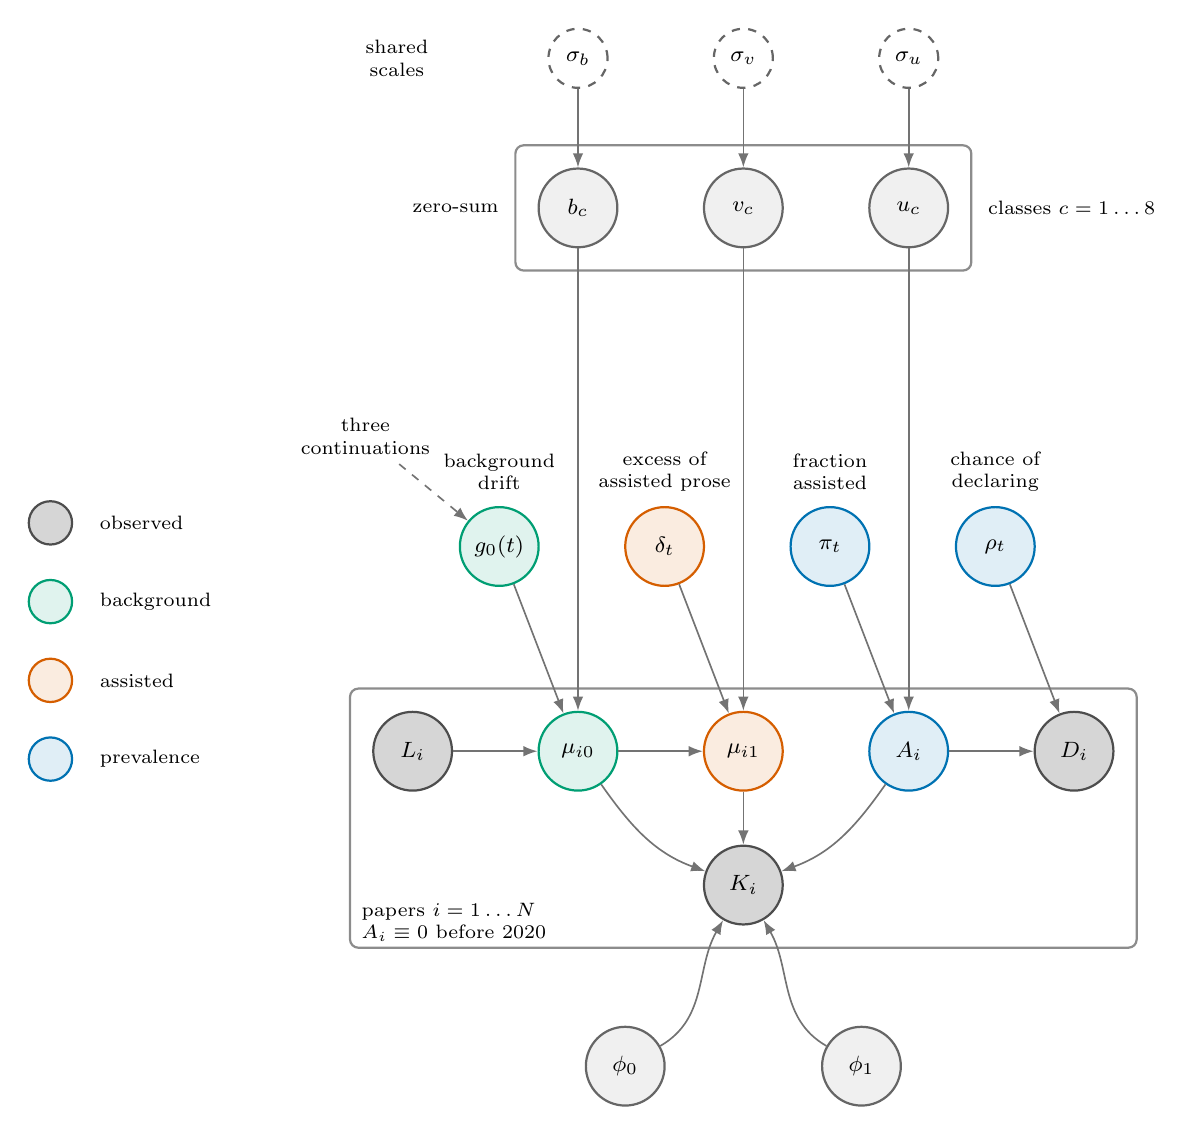
\begin{tikzpicture}[
    >={Latex[length=1.8mm]}, semithick, font=\small,
    node/.style={circle, thick, minimum size=10mm, align=center,
        inner sep=0.5pt, font=\footnotesize},
    bgN/.style={node, draw=oiGreen, fill=oiGreen!12},
    asN/.style={node, draw=oiOrange, fill=oiOrange!12},
    prN/.style={node, draw=oiBlue, fill=oiBlue!12},
    obs/.style={node, draw=oiGray, fill=black!16},
    plate/.style={rectangle, rounded corners=3pt, draw=black!45, thick,
        inner sep=8pt},
    platelab/.style={font=\scriptsize, text=black, align=left},
    edge/.style={->, draw=black!55},
    lab/.style={font=\scriptsize, text=black},
    newN/.style={node, draw=black!60, fill=black!6},
    hypN/.style={node, draw=black!60, fill=white, dashed, minimum size=7.5mm},
    newedge/.style={->, draw=black!55},
    newlab/.style={font=\scriptsize, text=black},
]

% shared scales (hyperparameters): the top of the hierarchy
\node[hypN] (sb) at (2.7, 9.4) {$\sigma_b$};
\node[hypN] (sv) at (4.8, 9.4) {$\sigma_v$};
\node[hypN] (su) at (6.9, 9.4) {$\sigma_u$};
\node[newlab, align=center] at (0.4, 9.4) {shared\\ scales};

% class plate (partial pooling across the eight subject classes)
\node[newN] (bc) at (2.7, 7.5) {$b_c$};
\node[newN] (vc) at (4.8, 7.5) {$v_c$};
\node[newN] (uc) at (6.9, 7.5) {$u_c$};
\begin{scope}[on background layer]
\node[plate, fit=(bc)(vc)(uc)] (cplate) {};
\end{scope}
\node[newlab, anchor=west] at ($(cplate.east)+(2pt,0)$) {classes $c=1\ldots8$};
\node[newlab, anchor=east, align=center] at ($(cplate.west)-(2pt,0)$)
    {zero-sum};

% quarter-level row
\node[bgN] (g0)    at (1.7, 3.2)  {$g_0(t)$};
\node[asN] (delta) at (3.8, 3.2)  {$\delta_t$};
\node[prN] (pi)    at (5.9, 3.2)  {$\pi_t$};
\node[prN] (rho)   at (8.0, 3.2)  {$\rho_t$};

\node[lab, align=center] at (1.7, 4.15)  {background\\ drift};
\node[lab, align=center] at (3.8, 4.15)  {excess of\\ assisted prose};
\node[lab, align=center] at (5.9, 4.15)  {fraction\\ assisted};
\node[lab, align=center] at (8.0, 4.15)  {chance of\\ declaring};

% paper plate
\node[obs] (L) at (0.6, 0.6)  {$L_i$};
\node[bgN] (mu0) at (2.7, 0.6) {$\mu_{i0}$};
\node[asN] (mu1) at (4.8, 0.6) {$\mu_{i1}$};
\node[prN] (A)  at (6.9, 0.6)  {$A_i$};
\node[obs] (K)  at (4.8, -1.1) {$K_i$};
\node[obs] (D)  at (9.0, 0.6) {$D_i$};
\begin{scope}[on background layer]
\node[plate, fit=(L)(mu0)(mu1)(A)(K)(D)] (pplate) {};
\end{scope}
\node[platelab, anchor=north west] at ($(pplate.south west)+(1pt,20pt)$)
    {papers $i=1\ldots N$\\ $A_i\equiv0$ before 2020};

% dispersions
\node[newN] (ph0) at (3.3, -3.4) {$\phi_0$};
\node[newN] (ph1) at (6.3, -3.4) {$\phi_1$};

% the three background continuations act here
\node[newlab, align=center] (var) at (0, 4.6) {three\\ continuations};
\draw[newedge, dashed] (var) -- (g0);

% edges
\draw[newedge] (sb) -- (bc);
\draw[newedge] (sv) -- (vc);
\draw[newedge] (su) -- (uc);
\draw[edge] (g0)    -- (mu0);
\draw[edge] (L)     -- (mu0);
\draw[edge] (mu0)   -- (mu1);
\draw[edge] (delta) -- (mu1);
\draw[edge] (pi)    -- (A);
\draw[edge] (rho)   -- (D);
\draw[edge] (mu0)   to[out=-55,in=160] (K);
\draw[edge] (mu1)   -- (K);
\draw[edge] (A)     to[out=-125,in=20] (K);
\draw[edge] (A)     -- (D);
\draw[newedge] (bc) -- (mu0);
\draw[newedge] (vc) -- (mu1);
\draw[newedge] (uc) -- (A);
\draw[newedge] (ph0) to[out=30,in=-120] (K);
\draw[newedge] (ph1) to[out=150,in=-60] (K);

% legend, placed clear of the plate label beneath the box
\node[obs, minimum size=5.5mm] at (-4,3.5) {};
\node[anchor=west, font=\scriptsize] at (-3.5,3.5) {observed};
\node[bgN, minimum size=5.5mm] at (-4,2.5) {};
\node[anchor=west, font=\scriptsize] at (-3.5,2.5) {background};
\node[asN, minimum size=5.5mm] at (-4,1.5) {};
\node[anchor=west, font=\scriptsize] at (-3.5,1.5) {assisted};
\node[prN, minimum size=5.5mm] at (-4,0.5) {};
\node[anchor=west, font=\scriptsize] at (-3.5,0.5) {prevalence};
\end{tikzpicture}
}
\caption{The hierarchical Bayesian model used in this work. Each paper contributes its analyzed length $L_i$, its marker count $K_i$, and its declaration flag $D_i$. The background rate $\mu_{i0}$ scales with length and drifts as $g_0(t)$. Assisted papers multiply that rate by the excess $e^{\delta_t}$, which we calibrate on the declared papers. The latent indicator $A_i$ has probability $\pi_t$, the quantity we report, and we fix it to zero before 2020. We suppress the topic effects, the overdispersion parameters, and the declared-versus-silent selection parameter in this figure and describe them in the text.\label{fig:model}}
\end{figure*}

For paper $i$ with analyzed length $L_i$, marker count $K_i$, and latent assistance indicator $A_i$, we write the counts as a two-component mixture of negative binomials,
\begin{align}
K_i \mid A_i{=}0 &\sim \mathrm{NB}(\mu_{i0},\,\phi_0),\nonumber\\
\log\mu_{i0} &= \log L_i + \beta_0 + b_{c_i} + g_0(t_i),\nonumber\\
K_i \mid A_i{=}1 &\sim \mathrm{NB}(\mu_{i1},\,\phi_1),\nonumber\\
\log\mu_{i1} &= \log\mu_{i0} + \delta_{t_i} + v_{c_i},\nonumber\\
A_i &\sim \mathrm{Bern}(\pi_{t_i,c_i}),\nonumber\\
\operatorname{logit}\pi_{t,c} &= m_t + u_c,
\label{eq:model}
\end{align}
and we fix $\pi\equiv0$ for papers submitted before 2020. Here $c_i$ is the broad topic class and $t_i$ the submission quarter. The terms $b_c$, $v_c$, and $u_c$ are partially pooled topic effects on the background, the excess, and the prevalence. The negative binomial dispersions $\phi_0$ and $\phi_1$ absorb the heavy tail that a Poisson model would misread as structure. Mixtures of this kind are routine for latent-class problems in astronomy \citep[e.g.][]{Hogg2010, Foreman-Mackey2014}.

Two features of Equation~\ref{eq:model} account for most of the improvement over the standard estimator. The first is the offset $\log L_i$, standard in count regression \citep{Cameron2013}. It makes our unit of evidence the count given length rather than the presence of a word anywhere in the document. The second is that we leave $\delta_t$ a free function of time, so the excess of assisted prose can fade as authors adapt without our reading that fading as a fall in use. We marginalize the latent $A_i$ analytically, so the fit involves only continuous parameters.

We treat declarations as positive-unlabeled labels \citep{Elkan2008}. A declaration is a positive, but its absence is not a negative, since most assisted authors say nothing. Writing $\rho_t$ for the probability that an assisted author declares, we let a declared paper contribute $\pi\rho\,p_1(K_i)$ and a silent paper contribute $(1-\pi)p_0(K_i)+\pi(1-\rho)p_1(K_i)$, where $p_0$ and $p_1$ are the two negative binomial densities.

\subsection{Identification and the counterfactual}\label{sec:m-ident}

Left to itself, a two-component mixture is a flexible curve fitter. Given any spread of counts it will find two components, whether or not two processes are really there. When we run our model on the neutral control basket with the excess left free, it does exactly that and reports a large prevalence for words that carry no signal. We take our remedy from the logic of the original spam filter \citep{Sahami1998}. We do not let the model invent the assisted component. We anchor it to the papers we know are assisted, by centering the prior on $\delta_t$ tightly on the marker excess that we measure in the declared papers themselves. Once we anchor it, the model has no way to turn ordinary drift in control words into prevalence.

We fix three other quantities from data rather than assume them. From the 106{,}000 pre-2020 papers we take the background level, how it scales with length, how it varies by topic, and how much it scatters. From the neutral controls we take a bound on how fast ordinary astronomy vocabulary drifts. From the declaration counts by year we take $\rho_t$. A fourth ingredient, the assumption that adoption only rises, is not data, and we report every
number without it as well.

One quantity we cannot fix by any of these means is the counterfactual from the introduction. We do not know what the background would have done after 2020 if chatbots had not been released. Rather than pick an answer and hide it, we fit the model three times. In the \textit{linear} variant we continue the trend we measure before 2020, which is what the standard estimator assumes. In the \textit{frozen} variant we hold the background at its 2020
level, so we attribute every later change to assistance, and this gives the highest answer. In the \textit{tracked} variant we tie the background to the measured drift of the neutral controls, and this gives the lowest. We take the spread between the three as our uncertainty, and after 2024 it is wider than the statistical error of any single fit.

\subsection{Inference and calibration}\label{sec:m-inf}

We maximize the log posterior on the unconstrained parametrization with exact gradients, and we take our uncertainties from the curvature at the mode, the Laplace approximation \citep[cf.][]{Gelman2013}. Every fit converges in about a minute, which is what makes the variant grid of Section~\ref{sec:m-robust} affordable. We check the approximation against full Hamiltonian Monte Carlo \citep{Neal2011, Hoffman2014, Betancourt2017} on the primary specification, and we check convergence with rank-normalized $\widehat{R}$ and effective sample size \citep{Vehtari2021}.

We calibrate the estimator on synthetic corpora that we build from the real pre-2020 papers, so that lengths, topics, and dispersion are realistic by construction, and we inject an assisted component at known prevalence and known excess. For excess factors of 2.5 and above we recover the prevalence to within two or three percentage points of the truth across the whole range. At an excess of 1.5 the degeneracy between prevalence and excess
widens and our scatter grows by an order of magnitude. This is the degeneracy that the monotonicity anchor exists to control. We measure a full-text excess near \observedExcess, inside the calibrated regime but not far from its edge, which is a further reason to quote the assumption bracket rather than the interval of any single fit.

% =====================================================================
\section{Results}\label{sec:results}

\begin{figure*}[!t]
\centering
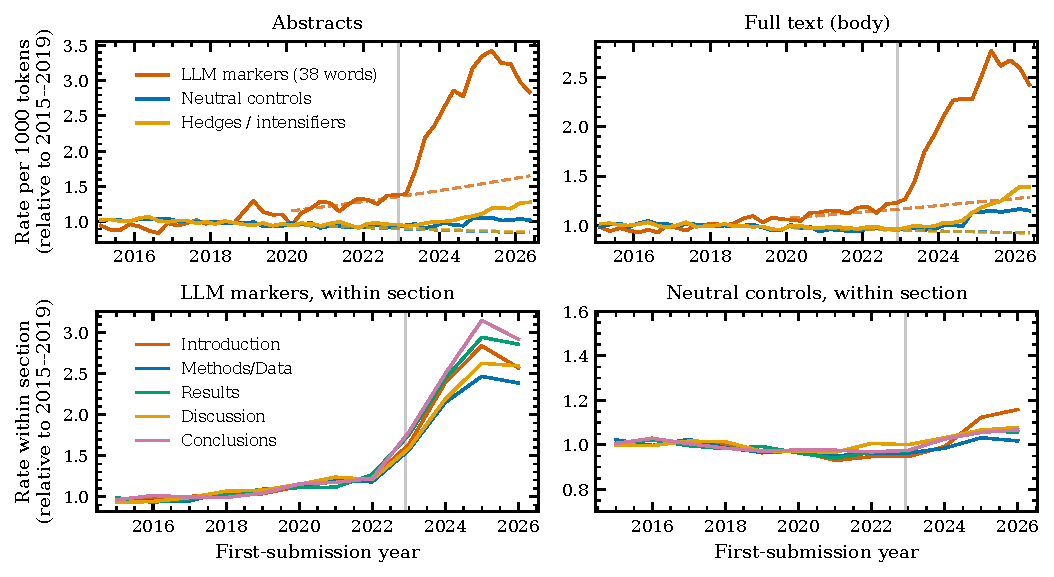
\includegraphics[width=\textwidth]{figs/fig1_composite.pdf}
\caption{We measure the occurrence rate of the three baskets across the decade, in abstracts and in full-text bodies. Top row, occurrence rate per 1000 tokens, normalized to 2015--2019. Dashed segments extend each basket's pre-2020 trend. The markers rise by a factor of \markerRiseFulltext\ in full text by 2025 while the per-token controls stay near flat. Bottom row, the same rates within each section. The marker rise appears in every section and the controls stay flat within every section, so the apparent control drift in whole-document counts comes mostly from section composition, with a small residual vocabulary drift that the model's background term absorbs. Dotted vertical lines mark the release of ChatGPT.\label{fig:rates}}
\end{figure*}

\subsection{A null test of the document-frequency estimator}\label{sec:placebo}

We apply the extrapolation estimator of \citet{Holzwarth2026} to the 38 markers on full text and obtain a 2025 assisted fraction of \betaMarkersFull. The estimator was built for abstracts, where a document is a few hundred tokens, and the failure we describe here is a failure of transfer to documents thirty times longer rather than of the arithmetic itself. On full text it does not survive our null test. When we apply the same arithmetic to the neutral control basket we obtain \ctrlBetaFull, and when we apply it to the null hedges we obtain a similar number. Words with no possible connection to language models therefore yield an apparent prevalence as large as the marker signal.

The mechanism is document length, since the median analyzed body grew from about 4{,}500 tokens in 2015 to 6{,}400 in 2025 and the probability that a fixed-rate word appears at least once rises with length. A statistic that asks only whether a word appears therefore reads longer papers as more contaminated. When we measure occurrences per token instead, most of the control excess disappears, as the top row of Figure~\ref{fig:rates} shows. On the per-token scale the markers rise by a factor of \markerRiseFulltext\ by 2025 while the controls stay near flat, and the small drift they retain is the ordinary-vocabulary change that the background term of our model absorbs.

The within-section panels rule out a second artifact, since the unlabeled share of the body shrinks over the decade and a whole-document rate therefore mixes a change of composition into the measurement. Within each of the five named sections we find the marker rise at similar strength, and within each section we find the controls flat. The rise is therefore a property of the prose rather than of which parts of papers the OCR labels.

\subsection{The assisted fraction}\label{sec:prevalence}

\begin{figure*}[!t]
\centering
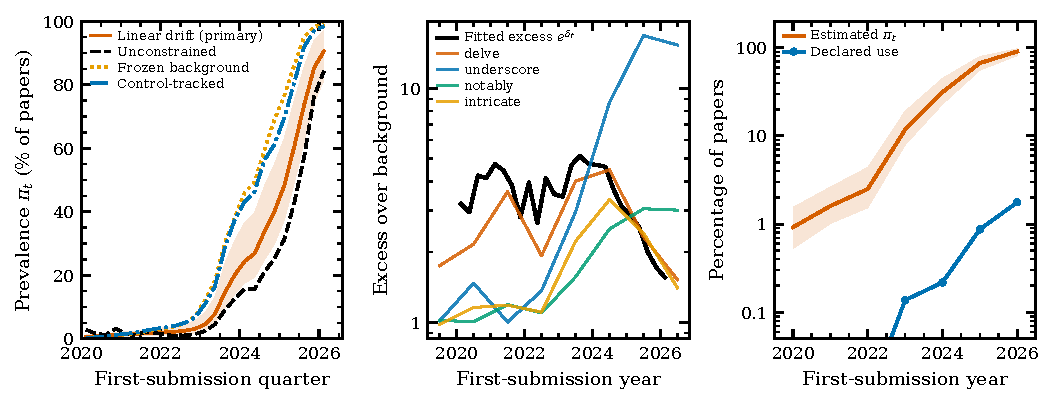
\includegraphics[width=\textwidth]{figs/fig3_composite.pdf}
\caption{We infer the assisted fraction by quarter and track how the excess of assisted prose changes as that fraction rises. Left, the assisted fraction by quarter. The band is our primary fit with its 95\% interval, and the other curves each change one assumption. The spread between the drift variants exceeds any single interval, and we take that spread as our uncertainty. Middle, the fitted excess of assisted prose falls while the prevalence rises. \textit{Delve} falls after mid-2024 while \textit{underscore} continues to rise, so fixed word lists lose power with time. Right, our estimated prevalence against declared use on a logarithmic scale.\label{fig:results}}
\end{figure*}

Our main result appears in Figure~\ref{fig:results}. Under the primary specification, the fraction of astro-ph papers whose analyzed prose shows a language-model trace reaches \piFulltextHeadline\ in 2025, up from \piFulltextTwentyFour\ in 2024. The three background counterfactuals give us the bracket \piFulltextBracket\ for 2025. The linear continuation sets the floor and the frozen background the ceiling, and the control-tracked variant falls between them. We read that ordering as informative in itself. The marker words were already drifting upward before 2020, so extrapolating that drift absorbs part of the post-2022 excess and gives us the most conservative answer. When we remove the monotonicity constraint the 2025 figure falls to \piUnconstrained.

The estimand we adopt is deliberately modest, the fraction of papers whose analyzed prose is more consistent with our calibrated assisted component than with the background. This is weaker than the claim that a machine wrote the paper and stronger than the observation that a paper contains one suspicious word. We count an author who ran a single section through a chatbot for grammar. We do not count model use that leaves no lexical trace, whether because the author edited it away or because the help was with code or ideas rather than prose. Every number we report is a floor in that sense. We treat the per-paper posterior probabilities as latent weights for aggregation and we do not publish them.

\subsection{Time evolution of the marker excess}\label{sec:fading}

The middle panel of Figure~\ref{fig:results} shows our second result. We find that the fitted excess of assisted prose falls from \deltaEarly\ times the background in 2023 to \deltaLate\ by 2026 while the prevalence rises. Taken together, these two motions are the population-level form of the adjustment that \citet{Geng2025} measured word by word. More papers pass through models while each leaves a fainter lexical trace.

\begin{figure*}[!t]
\centering
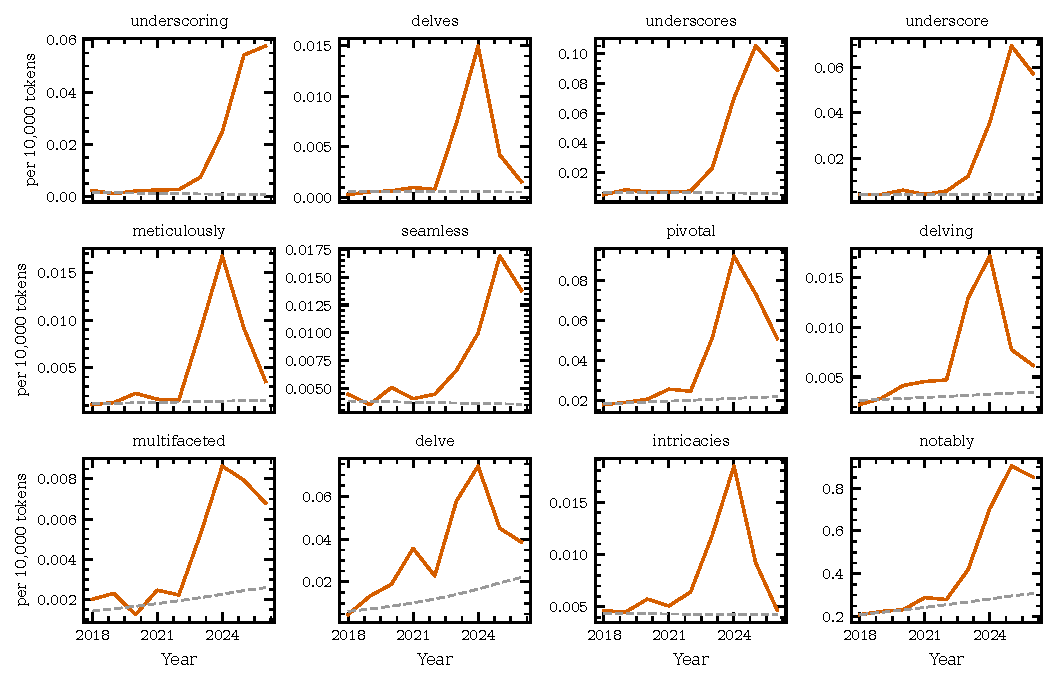
\includegraphics[width=\textwidth]{figs/fig3_marker_trajectories.pdf}
\caption{We follow each marker word separately to show that the aggregate signal is steadier than any of its parts. Observed occurrence rate (red) of the twelve markers with the largest recent excess, against the background that we extrapolate from before 2020 (dashed). We deconvolve the rates against the fitted prevalence, so no word selects the papers that we use to measure that word. The words do not move together, since \textit{delve} peaks in 2024 and returns toward its baseline while \textit{underscore} and \textit{notably} are still rising in 2026. This is why an estimator tied to a fixed word list loses power while one that lets the excess move does not.\label{fig:words}}
\end{figure*}

In Figure~\ref{fig:words} we show the same result one word at a time. We compute the per-word curves by deconvolution against the fitted prevalence, so that no word selects the papers that we use to measure that word. \textit{Delve} falls after mid-2024, when it became a widely recognized tell, while \textit{underscore} and \textit{notably} continue to rise. The practical implication is that fixed word lists lose their power within a few years, and any estimator that holds the excess constant will read the fading of markers as a fall in use.

\subsection{A marker vocabulary derived from the astronomy corpus}\label{sec:discovery}

\begin{figure*}[!t]
\centering
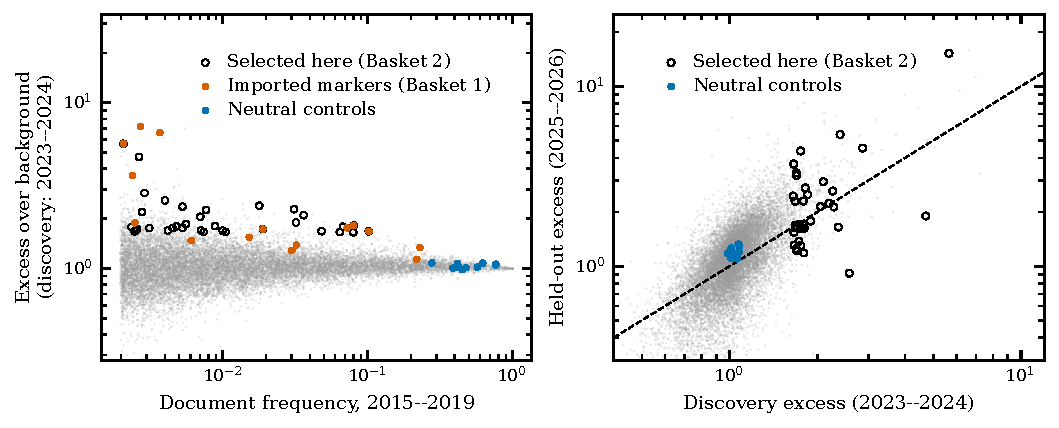
\includegraphics[width=\textwidth]{figs/fig4_composite.pdf}
\caption{We derive a marker vocabulary from the astronomy corpus itself and test it on years the selection never saw. \texttt{Left:} every word with a stable pre-2020 background, placed by its 2015--2019 document frequency and its 2023--2024 excess over the extrapolated background. Circled words pass our selection screen, which requires a stable background, a rise in the discovery years, and a spread across all eight topic classes. The last criterion separates writing style from subfield vocabulary. \texttt{Right:} the frozen selection evaluated on 2025--2026. The selected words scatter about the dashed one-to-one line while the neutral controls cluster at unit excess on both axes.\label{fig:discovery}}
\end{figure*}

We imported the 38-word basket from other fields, and language models may mark astronomy prose differently. We therefore derive a second basket from the corpus itself, using a temporal split that we fix in extend. We require a candidate to occur in at least 0.2\% of pre-2020 papers with a stable background, to rise by at least 60 per cent over the extrapolated background in the discovery years 2023 and 2024, and to spread across all eight topic classes. The last requirement separates writing style, which appears in every subfield at once, from science, which does not. The same screen that promotes \textit{noteworthy} and \textit{comprehensively} rejects the pulsar-timing vocabulary that rose sharply after the 2023 gravitational-wave background detections. We remove author-name fragments and facility names with a dictionary requirement and a short stoplist. The selected words appear in Table~\ref{tab:baskets}.

Our frozen basket has \nExpandedWords\ words, of which \nExpandedNew\ are new relative to the seeds. Of these, \nExpandedHeld\ independently show more than 20\% excess in 2025 and 2026, years that our selection never used, and the neutral controls pass the same screen at ratios between 0.98 and 1.08. When we fit the model with this basket we obtain \piExpandedHeadline\ for 2025 under linear drift and \piExpandedTracked\ under tracked drift, both inside the bracket that we obtained with the imported words. We regard the agreement as more informative than either value. Two marker vocabularies with different origins, one imported from biomedical and computer-science studies and one that we discovered here under a split fixed in extend, place the 2025 fraction in the same range.

\begin{deluxetable*}{llcl}
\tablecaption{The marker, control, and null vocabularies.\label{tab:baskets}}
\tablehead{\colhead{Basket} & \colhead{Class} & \colhead{$N$} & \colhead{Words}}
\startdata
Basket 1, imported & Strong tells & 18 & \parbox[t]{0.455\textwidth}{\raggedright \textit{boasts, delve, delves, delving, intricacies, intricate, meticulous, meticulously, nuanced, pivotal, realm, realms, showcases, showcasing, tapestry, underscore, underscores, underscoring}} \\[4pt]
Basket 1, imported & Soft tells & 20 & \parbox[t]{0.455\textwidth}{\raggedright \textit{comprehensive, crucial, elucidate, encompass, encompasses, garner, harness, harnessing, holistic, insights, leverage, leveraging, multifaceted, myriad, notably, plethora, robust, seamless, seamlessly, unravel}} \\[4pt]
Basket 2, astronomy-native & Screened & 35 & \parbox[t]{0.455\textwidth}{\raggedright \textit{adhere, align, attribution, categorize, commence, comprehend, comprehension, comprehensive, comprehensively, conversely, disparity, disregard, elucidate, examining, exceeding, excessively, gratitude, grounded, hinge, luckily, nonexistent, notably, noteworthy, offering, penultimate, posit, readability, refining, seeming, situated, stood, substantiate, surpass, underscore, utilize}} \\[4pt]
Controls & Neutral & 10 & \parbox[t]{0.455\textwidth}{\raggedright \textit{galaxy, measured, observed, obtained, presented, redshift, sample, spectra, stellar, temperature}} \\[4pt]
Null hedges & Frequency-matched & 15 & \parbox[t]{0.455\textwidth}{\raggedright \textit{adequate, apparent, considerable, consistent, corresponding, derived, distinct, estimated, evident, moderate, notable, reliable, significant, substantial, typical}} \\[4pt]
\enddata
\tablecomments{Basket 1 carries the words imported from the corpus studies of other
fields, separated into strong tells that stay rare in astronomy prose and soft
tells that hold everyday scientific uses. Basket 2 carries the words that the
frozen temporal screen of Section~\ref{sec:discovery} draws from the astronomy
corpus itself, of which 31 are new relative to Basket 1. The controls anchor the
background rate and the null hedges match the marker frequency distribution
without carrying any tell.}
\end{deluxetable*}


\subsection{Robustness of the estimate}\label{sec:m-robust}

The claim we defend is the floor rather than the central value. We therefore relax the standard estimator's restrictions one at a time, in four steps, so that the effect of each assumption stays visible rather than bundled into the end point. Step 1 is the standard estimator itself, which counts document frequency and gives \ladderFullRungZero. Step 2 measures occurrences per token against a flat background and anchors the excess on the declared papers, which gives \ladderFullRungTwo. Step 3 lets that background drift and gives \ladderFullRungThree. Step 4 is the full hierarchy, which gives the posterior \ladderFullRungFour.

Across these steps the marker estimates rise rather than fall, because at full-text lengths the document-frequency statistic saturates and under-reads the excess. The neutral controls move the other way, giving a spurious \ladderCtrlRungZero\ at step 1 and losing any defined value from step 2 onward, because declared papers use control words at the background rate and the estimator therefore reports that those words carry no signal.

We run five checks to bound the answer. First, in the anchored model the control words yield an attributed excess of \ctrlExcessRate\ of their own background, consistent with the measured drift of ordinary vocabulary and an order of magnitude below the \markerExcessRate\ that we attribute for markers. Second, we find that the simplest defensible estimator agrees with the full one. Step 2 is a single line of arithmetic, the observed per-token excess divided by the excess that we measure in declared papers, and it gives \ladderFullRungTwo\ with no hierarchy at all. Third, we find that the vocabulary does not drive the answer, as Section~\ref{sec:discovery} shows. Fourth, we move the known-negative boundary from 2020 to the quarter before the public release of ChatGPT, which changes the 2025 estimate by \boundaryShift, and we rescale the declared-to-silent marker-rate ratio by a factor of two in either direction, which moves it by up to \gammaShift. These are our largest systematics after the drift bracket, and both leave the floor intact. Fifth, our pipeline reproduces known answers on synthetic corpora, as we describe in Section~\ref{sec:m-inf}.

The one scenario that would break our conclusion is a large, marker-specific shift in human vocabulary that began exactly when chatbots launched, affected every section and every topic class at once, and left the neutral controls untouched, in which case we would misread it as model use. We cannot exclude that scenario on logical grounds. We can say that our control and null baskets were built to catch it, and that they show \ctrlExcessRate.

\subsection{Comparison with declared use}\label{sec:gap}

We find declared use two orders of magnitude below estimated use. In 2025, \declRateTwentyFive\ of full texts contain an explicit declaration against an estimated prevalence of \piFulltextHeadline, so roughly \disclosureGapFactor\ papers carry a language-model trace for every one that says so. The gap shows no sign of closing, since declarations grew by a factor of four between 2023 and 2025 and our estimated prevalence grew faster.

% =====================================================================
\section{Discussion}\label{sec:discussion}

We find that more than half of recent astro-ph papers carry a language-model trace in their prose. Our 2025 fraction is \piFulltextHeadline\ under the primary specification, and it never falls below \piGridFloor\ across the variants we ran. Astronomy therefore sits near the 89 per cent that \citet{Holzwarth2026} report for biomedicine and well above the few-per-cent figures that circulate from abstract-only studies.

Abstracts, run through the same model, give \piAbstractsHeadline\ for 2025, consistent with our full-text bracket. We read the apparent order-of-magnitude disagreement between abstract and full-text estimates in the earlier literature as an artifact of comparing a 200-token document with a 2{,}500-token one using a statistic that saturates with length. Once we measure counts per token and calibrate the assisted component separately in each corpus, the two agree. Abstracts remain the weaker instrument, and our intervals from them are roughly twice as wide because each paper offers thirty times fewer tokens.

Our conclusions carry three limitations. First, our estimand is a trace in analyzed prose, so we cannot see use that leaves no lexical trace, and every number we report is a floor. Second, we work from OCR text of the latest revision of each paper, so our known-negative era can contain a small admixture of post-2022 revisions, which we bound with the boundary test at \boundaryShift. Third, we calibrate the assisted component on declared papers, a selected minority, and we span the plausible selection with the $\gamma$ sweep at \gammaShift. That sweep is a span rather than a measurement, because the comparison it stands in for, the marker rate of authors who used a model and did not say so, is by definition unobserved.

A fourth limit applies to every method in this literature, ours included. When the assisted and background components sit close together, a small error in the background counterfactual becomes a large error in the fraction. For vocabulary with a strong excess, such as our markers, this does little damage. For vocabulary with a weak excess it removes the answer entirely, and more data does not help. This is why we report the null test in units of excess rate rather than as a prevalence, and why we would not trust a prevalence built on low-excess words, whoever computed it.

We do not read our result as misconduct at scale. The lexical shift is strongest in the writing of non-native English speakers, where others have read it as a leveling of linguistic barriers rather than as misconduct \citep{Lin2025}, and much of what we detect is likely the grammar and style assistance that journal policies already permit. The problem we see is the factor of \disclosureGapFactor\ between practice and disclosure. A policy that most of a field quietly ignores does not deliver the transparency it was written for.

Two consequences follow for policy. First, enforcement built on detection has a limited future. We measure the excess falling from \deltaEarly\ to \deltaLate\ within three years while use rises, so any fixed vocabulary loses power, and a policy that depends on catching offenders will fail while the behaviour it targets grows. Disclosure norms that authors have a reason to follow will outlast detection. Second, the window for this measurement is closing, since if the trace continues to fade at the rate we measure, corpus-level estimates of this kind will become unreliable within a few years, and nobody can recreate the pre-2023 baseline that makes them possible. We therefore argue for measuring now, and for archiving the corpora and the marker vocabularies that later work will need in order to check us.

\section*{Acknowledgments}

SMS is supported by the Distinguished University Fellowship awarded by The Ohio State University. YST is supported by NSF under Grant AST-2406729 and by a Humboldt Research Award from the Alexander von Humboldt Foundation.

We built this work on the AstroMLab~5 astro-ph catalog and its companion $n$-gram index.

Given the subject of this paper, we state our own practice plainly. We used Claude Code for coding development. We drafted and revised the text ourselves, then we use Claude Opus 5 for editing the prose and grammar throughout the paper.

\section*{Data and code availability}

The corpus is the public AstroMLab~5 catalog \citep{Ting2025}. We release the derived per-paper feature tables, the frozen baskets, the fitted posteriors, and all analysis code with this paper. We do not release a per-paper assisted-probability list.









\software{NumPy \citep{2020Natur.585..357H}, SciPy
\citep{2020NaMet..17..261V}, Matplotlib \citep{2007CSE.....9...90H}, pandas
\citep{2020zndo...3509134R}, JAX \citep{jax2018github}, PyMC
\citep{2023PeerJCS...9.1516A}, ArviZ \citep{2019JOSS....4.1143K}}

\bibliographystyle{aasjournal}
\bibliography{refs}

\end{document}
